\documentclass[12pt,a4paper]{article}

\usepackage[utf8]{inputenc}
\usepackage[T1]{fontenc}
\usepackage[french]{babel}
\usepackage{graphicx}
\usepackage{hyperref}
\usepackage{geometry}
\usepackage{xcolor}
\usepackage{listings}
\usepackage{booktabs}
\usepackage{setspace}
\usepackage{tocloft}
\usepackage{float}
\usepackage{amsmath}
\usepackage{enumitem}
\usepackage{longtable}

\geometry{margin=2.5cm}
\setstretch{1.2}

\definecolor{codegreen}{rgb}{0,0.6,0}
\definecolor{codegray}{rgb}{0.5,0.5,0.5}
\definecolor{codepurple}{rgb}{0.58,0,0.82}
\definecolor{backcolour}{rgb}{0.95,0.95,0.92}

\lstdefinestyle{mystyle}{
    backgroundcolor=\color{backcolour},   
    commentstyle=\color{codegreen},
    keywordstyle=\color{magenta},
    numberstyle=\tiny\color{codegray},
    stringstyle=\color{codepurple},
    basicstyle=\ttfamily\footnotesize,
    breakatwhitespace=false,         
    breaklines=true,                 
    captionpos=b,                    
    keepspaces=true,                 
    numbers=left,                    
    numbersep=5pt,                  
    showspaces=false,                
    showstringspaces=false,
    showtabs=false,                  
    tabsize=2
}
\lstset{style=mystyle}

\title{\Huge\textbf{Rapport de Projet}\\[0.5cm]
\Large\textbf{Conception, Implémentation et Évaluation d'un Système d’Audit et de Supervision de Sécurité sous Linux}}
\author{\textbf{OSS}\\Taha Hanaa Amira \\ Taha Wahiba \\ ING4 SECI }
\date{\today}

\begin{document}

\begin{titlepage}
    \maketitle
    \vfill
    \begin{abstract}
    Ce rapport présente la conception, l’implémentation et l’évaluation d’un système léger d’audit et de supervision de sécurité dédié aux systèmes GNU/Linux. La solution repose sur l’exploitation coordonnée de mécanismes natifs du système d’exploitation, tels que \texttt{auditd}, \texttt{rsyslog} et les journaux d’authentification, ainsi que sur une application Python/Flask développée pour collecter, structurer et visualiser les événements sensibles. Le système permet notamment la détection des tentatives d’authentification SSH échouées, de l’usage de privilèges élevés via \texttt{sudo}, de l’ouverture de sessions privilégiées et de l’accès à des fichiers critiques comme \texttt{/etc/passwd} et \texttt{/etc/shadow}. L’ensemble constitue une solution reproductible, cohérente et concrète pour illustrer le rôle de l’audit système dans la sécurité des systèmes d’exploitation.
    \end{abstract}
    \vfill
\end{titlepage}

\newpage
\tableofcontents
\newpage

\section{Introduction et Objectifs}

\subsection{Contexte général de la cybersécurité système}

La sécurité des systèmes d’exploitation est aujourd’hui un enjeu central dans l’administration des infrastructures numériques. Les systèmes GNU/Linux sont massivement utilisés pour l’hébergement de services critiques, le déploiement d’applications cloud, l’exécution de serveurs web, la virtualisation et les environnements de recherche. Cette omniprésence les rend naturellement attractifs pour les attaquants.

Les menaces pesant sur un système Linux sont multiples :
\begin{itemize}
    \item tentatives d’accès non autorisé à distance ;
    \item élévations de privilèges ;
    \item altération des fichiers système ;
    \item compromission d’identités locales ;
    \item effacement ou dissimulation des traces d’activité.
\end{itemize}

Dans ce contexte, la simple prévention ne suffit pas. Un système doit aussi être capable de \textbf{journaliser}, \textbf{tracer}, \textbf{détecter} et \textbf{présenter} les événements de sécurité de manière intelligible. C’est précisément sur ce besoin que s’inscrit ce projet.

\subsection{Problématique}

Les journaux Linux fournissent une richesse d’information considérable, mais ils sont dispersés, verbeux et difficiles à exploiter manuellement. Un administrateur qui consulte uniquement \texttt{/var/log/auth.log} ou la sortie brute de \texttt{ausearch} doit effectuer lui-même l’analyse, la corrélation et l’interprétation de chaque événement. Cette démarche est fastidieuse, peu ergonomique, et peu adaptée à un suivi rapide de l’état de sécurité d’un système.

La problématique principale du projet peut donc être formulée ainsi :

\begin{quote}
Comment concevoir une solution légère, locale et reproductible permettant d’exploiter les mécanismes natifs d’audit de Linux afin de détecter et visualiser rapidement des événements sensibles du système d’exploitation ?
\end{quote}

\subsection{Objectifs du projet}

Les objectifs techniques et pédagogiques du projet sont les suivants :
\begin{itemize}
    \item mettre en place un environnement expérimental reproductible ;
    \item exploiter le module d’audit du système d’exploitation ;
    \item collecter les traces liées à l’authentification et à l’intégrité des fichiers critiques ;
    \item structurer ces événements sous forme d’alertes exploitables ;
    \item développer un tableau de bord permettant une lecture centralisée ;
    \item démontrer la pertinence du dispositif à travers des scénarios de test concrets.
\end{itemize}

\section{État de l’art}

\subsection{Journalisation système sous Unix et Linux}

Historiquement, les systèmes Unix et Linux ont toujours accordé une place importante à la journalisation. Le paradigme selon lequel chaque événement significatif doit laisser une trace exploitable a conduit à l’émergence de plusieurs briques fondamentales :
\begin{itemize}
    \item \texttt{syslog} et ses implémentations modernes comme \texttt{rsyslog} ;
    \item \texttt{journald} dans les environnements basés sur \texttt{systemd} ;
    \item les journaux applicatifs spécialisés, tels que \texttt{auth.log}.
\end{itemize}

Ces outils permettent la conservation des événements, mais ils ne fournissent pas toujours de mécanisme d’analyse orienté sécurité. Une ligne de log n’est qu’une donnée brute ; elle ne devient utile que si elle est interprétée dans un contexte d’audit ou de supervision.

\subsection{Le module d’audit du système d’exploitation}

L’un des composants les plus importants de la sécurité Linux est le \textbf{Linux Audit System}, généralement utilisé à travers le démon \texttt{auditd}. Contrairement à un simple mécanisme de journalisation applicative, \texttt{auditd} repose sur une interaction avec le noyau Linux et permet d’observer des événements critiques au niveau des accès et des opérations sensibles.

Le module d’audit apporte plusieurs garanties fondamentales :
\begin{itemize}
    \item traçabilité des événements critiques ;
    \item possibilité de définir des politiques d’observation très précises ;
    \item corrélation entre utilisateur, action, cible et horodatage ;
    \item exploitation post-incident via des outils comme \texttt{ausearch}.
\end{itemize}

Du point de vue de la sécurité des systèmes d’exploitation, \texttt{auditd} joue donc le rôle d’un \textbf{module de preuve et de surveillance}, complémentaire aux mécanismes de permissions, d’authentification et de contrôle d’accès.

\subsection{Solutions existantes du marché}

Des solutions plus complètes comme Wazuh, Splunk ou Elastic Security permettent d’aller beaucoup plus loin en matière de corrélation, de centralisation et de détection avancée. Néanmoins, ces plateformes sont souvent lourdes, complexes à déployer, et peu adaptées à un projet académique centré sur la compréhension du fonctionnement interne du système.

L’intérêt de notre projet est justement de construire une solution plus légère, afin de comprendre les briques essentielles :
\begin{itemize}
    \item collecte des événements ;
    \item traitement ;
    \item stockage ;
    \item restitution.
\end{itemize}

\section{1.1 Environnement expérimental}

\subsection{Plateforme reproductible}

L’expérimentation a été réalisée dans un environnement virtualisé afin de garantir la reproductibilité, l’isolation des tests et la maîtrise de la configuration logicielle. Le projet a été déployé sur une seule machine virtuelle exécutant Kali Linux.

Le choix d’une seule machine virtuelle permet :
\begin{itemize}
    \item de simplifier l’architecture du projet ;
    \item de réduire les ressources nécessaires ;
    \item de faciliter la démonstration dans un contexte académique ;
    \item de rendre la reproduction plus accessible.
\end{itemize}

\subsection{Architecture retenue}

L’architecture retenue repose sur une approche \textbf{single-host}, c’est-à-dire une solution entièrement exécutée sur une seule machine virtuelle Kali Linux.

Cette machine regroupe :
\begin{itemize}
    \item le système cible à surveiller ;
    \item le module d’audit \texttt{auditd} ;
    \item les journaux système, notamment \texttt{/var/log/auth.log} ;
    \item l’application Python de collecte et de traitement ;
    \item la base de données SQLite ;
    \item le serveur Flask assurant l’interface Web de supervision.
\end{itemize}

\subsection{Description précise de l’architecture}

Le fonctionnement général du système est le suivant :
\begin{enumerate}
    \item Kali Linux génère des événements système lors des actions sensibles ;
    \item les événements d’authentification sont enregistrés dans \texttt{/var/log/auth.log} ;
    \item les accès à certains fichiers critiques sont capturés par \texttt{auditd} ;
    \item l’application Python lit périodiquement ces deux sources ;
    \item les événements détectés sont transformés en alertes structurées ;
    \item les alertes sont enregistrées dans une base SQLite locale ;
    \item le dashboard Flask interroge cette base et affiche les alertes en temps réel ou quasi temps réel.
\end{enumerate}
\section{1.2 Partie analyse}

\subsection{Présentation du problème de sécurité}

Le problème traité concerne la difficulté de superviser efficacement certains événements système particulièrement sensibles :
\begin{itemize}
    \item tentatives de connexion SSH échouées ;
    \item usage de privilèges administrateur ;
    \item ouverture de session root ;
    \item modification ou accès à des fichiers d’identité ;
    \item opérations affectant les comptes utilisateurs.
\end{itemize}

Ces événements ne sont pas forcément bloqués par défaut, mais ils doivent être au minimum \textbf{visibles} et \textbf{tracés}.

\subsection{Compréhension du fonctionnement interne du système d’exploitation}

Le projet a nécessité de comprendre plusieurs mécanismes internes du système Linux :

\begin{itemize}
    \item \textbf{PAM} : gère l’authentification et l’ouverture des sessions ;
    \item \textbf{sshd} : enregistre les connexions distantes et leurs échecs ;
    \item \textbf{sudo} : élève temporairement les privilèges ;
    \item \textbf{auditd} : consigne des événements liés aux fichiers, permissions et opérations sensibles ;
    \item \textbf{rsyslog} : centralise les journaux dans des fichiers persistants.
\end{itemize}

Le projet s’appuie donc directement sur des modules réels du système d’exploitation et non sur une simple couche applicative abstraite.

\subsection{Identification des risques}

Les principaux risques identifiés sont :
\begin{itemize}
    \item \textbf{bruteforce SSH} : un attaquant tente plusieurs connexions avec différents utilisateurs ou mots de passe ;
    \item \textbf{élévation de privilèges} : un utilisateur exécute des commandes sensibles via \texttt{sudo} ;
    \item \textbf{compromission des identités} : des fichiers comme \texttt{/etc/passwd} ou \texttt{/etc/shadow} sont accédés ou modifiés ;
    \item \textbf{insuffisance de visibilité} : les administrateurs ne disposent pas d’un point de vue synthétique sur les événements critiques.
\end{itemize}

\section{1.3 Partie implémentation}

\subsection{Vue d’ensemble de l’implémentation}

La solution développée comprend :
\begin{itemize}
    \item un programme Python principal \texttt{app.py} ;
    \item une base de données SQLite nommée \texttt{security\_events.db} ;
    \item des routes Flask pour exposer les alertes ;
    \item des règles permanentes \texttt{auditd} ;
    \item une interface Web de dashboard.
\end{itemize}

\subsection{Configuration de l’audit}

Les règles d’audit sont définies dans un fichier \texttt{security.rules} qui doit être copié dans le répertoire des règles permanentes :

\begin{lstlisting}[language=bash, caption=Déploiement de la configuration d’audit]
sudo cp config/security.rules /etc/audit/rules.d/
sudo augenrules --load
sudo systemctl restart auditd
sudo auditctl -l
\end{lstlisting}

Exemple de règles utilisées :

\begin{lstlisting}[language=bash, caption=Règles d’audit pour les fichiers sensibles]
-w /etc/passwd -p wa -k identity
-w /etc/shadow -p wa -k identity
-w /etc/group -p wa -k identity
-w /etc/gshadow -p wa -k identity
\end{lstlisting}

Ces règles associent la clé \texttt{identity} aux événements concernant les fichiers critiques du système.

\subsection{Collecte depuis \texttt{/var/log/auth.log}}

Le fichier \texttt{/var/log/auth.log} est utilisé pour détecter :
\begin{itemize}
    \item les échecs d’authentification SSH ;
    \item les commandes exécutées avec \texttt{sudo} ;
    \item l’ouverture d’une session privilégiée root.
\end{itemize}

Une partie essentielle de l’implémentation repose sur des expressions régulières capables d’identifier des motifs précis dans les logs système. Cela permet de transformer des lignes brutes en événements structurés.

\subsection{Collecte depuis \texttt{auditd}}

La surveillance des fichiers sensibles s’effectue par interrogation périodique de :

\begin{lstlisting}[language=bash, caption=Interrogation des événements d’audit]
ausearch -k identity -m PATH -i -ts recent
\end{lstlisting}

Cette commande permet d’extraire les événements récents correspondant à la clé \texttt{identity}. Les résultats sont ensuite convertis en alertes de type \texttt{FILE}.

\subsection{Stockage des alertes}

Les alertes sont stockées dans SQLite avec plusieurs attributs :
\begin{itemize}
    \item identifiant ;
    \item horodatage ;
    \item source ;
    \item type d’événement ;
    \item sévérité ;
    \item titre ;
    \item description ;
    \item log brut.
\end{itemize}

Cette structure permet d’obtenir à la fois un stockage léger et une restitution claire dans le tableau de bord.

\subsection{Dashboard et routes API}

L’interface Web repose sur Flask et met à disposition :
\begin{itemize}
    \item \texttt{/api/v1/system} : métriques système ;
    \item \texttt{/api/v1/alerts} : dernières alertes ;
    \item \texttt{/api/v1/stats} : statistiques agrégées ;
    \item \texttt{/api/v1/chart} : données pour graphique ;
    \item \texttt{/} : interface principale.
\end{itemize}

\subsection{Représentation des événements système}

La figure suivante illustre la représentation des événements système collectés et analysés par le dispositif.

\begin{figure}[H]
    \centering
    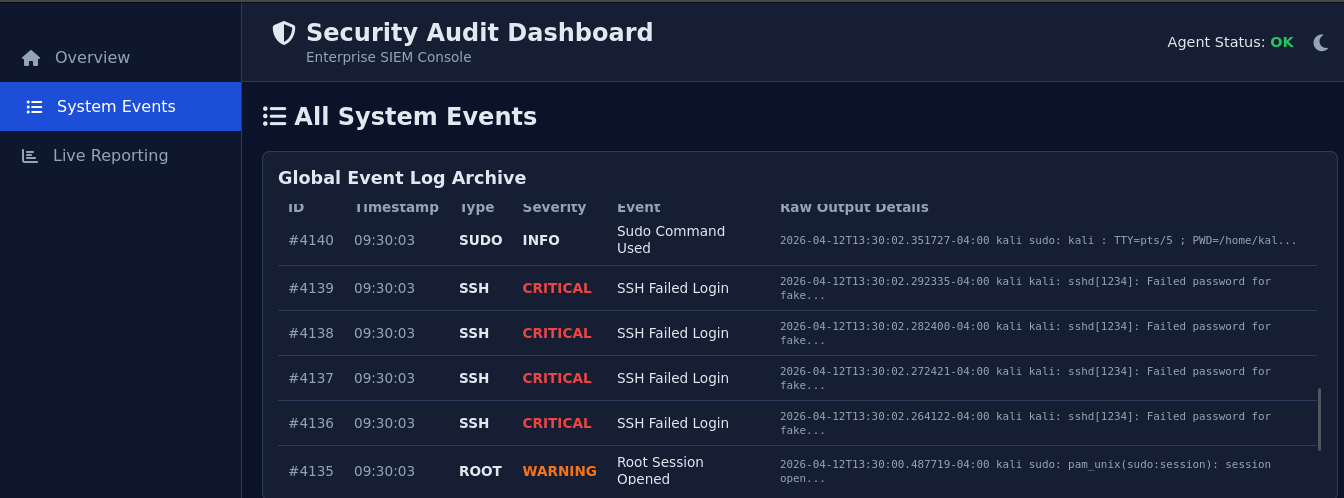
\includegraphics[width=0.92\textwidth]{image1.png}
    \caption{Représentation des événements système détectés}
    \label{fig:image1}
\end{figure}

\subsection{Visualisation dans le dashboard}

La figure suivante présente le dashboard développé pour la supervision des alertes.

\begin{figure}[H]
    \centering
    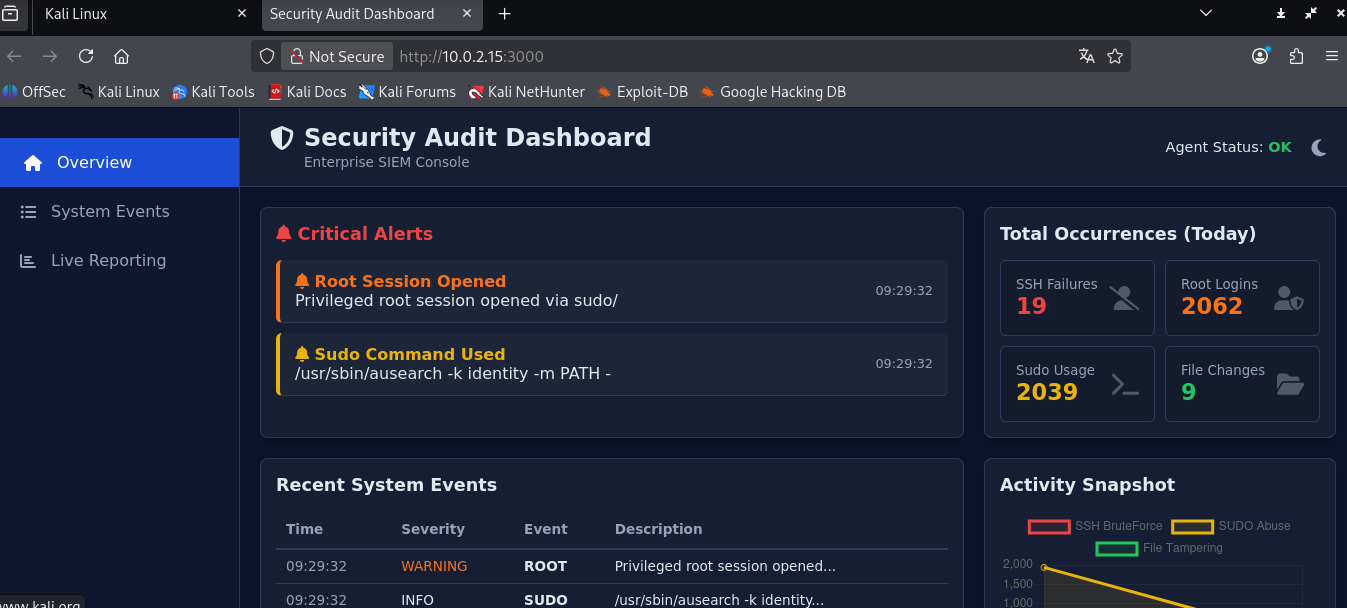
\includegraphics[width=0.92\textwidth]{image2.png}
    \caption{Dashboard Web de supervision de sécurité}
    \label{fig:image2}
\end{figure}

\section{1.4 Expérimentation}

\subsection{Scénarios de test}

Plusieurs scénarios ont été exécutés afin de valider la solution.

\subsubsection{Scénario 1 : tentative SSH échouée}

Commande :
\begin{lstlisting}
ssh fakeuser@localhost
\end{lstlisting}

Objectif :
\begin{itemize}
    \item générer une ligne de type \texttt{Failed password} ;
    \item vérifier la détection dans \texttt{auth.log} ;
    \item observer la remontée de l’alerte dans le dashboard.
\end{itemize}

\subsubsection{Scénario 2 : utilisation de sudo}

Commande :
\begin{lstlisting}
sudo ls /root
\end{lstlisting}

Objectif :
\begin{itemize}
    \item générer un événement \texttt{sudo} ;
    \item tracer l’ouverture d’une session privilégiée ;
    \item vérifier la visualisation dans l’interface.
\end{itemize}

\subsubsection{Scénario 3 : accès à un fichier sensible}

Commande :
\begin{lstlisting}
sudo touch /etc/passwd
\end{lstlisting}

Objectif :
\begin{itemize}
    \item déclencher une règle \texttt{auditd} ;
    \item vérifier la présence de l’événement via \texttt{ausearch} ;
    \item observer la création d’une alerte \texttt{FILE}.
\end{itemize}

\subsubsection{Scénario 4 : opération sur les identités}

Commande :
\begin{lstlisting}
echo "hacker_test:newpass" | sudo chpasswd
\end{lstlisting}

Objectif :
\begin{itemize}
    \item simuler une modification sensible concernant un utilisateur local ;
    \item enrichir l’analyse des actions sur l’identité.
\end{itemize}

\subsection{Comparaison avant / après}

\begin{table}[H]
\centering
\begin{tabular}{@{}p{4.8cm}p{5cm}p{5cm}@{}}
\toprule
\textbf{Indicateur} & \textbf{Avant la solution} & \textbf{Après implémentation} \\
\midrule
Lecture des événements & Fichiers de logs dispersés & Vue centralisée via dashboard \\
Détection des usages sudo & Lecture manuelle nécessaire & Alerte structurée en base \\
Surveillance fichiers sensibles & Peu visible à l’œil nu & Détection via auditd + visualisation \\
Exploitation pédagogique & Complexe & Lisible et démontrable \\
\bottomrule
\end{tabular}
\caption{Comparaison avant / après mise en place du système}
\end{table}

\subsection{Preuves de fonctionnement}

Les preuves de fonctionnement reposent sur plusieurs niveaux :
\begin{itemize}
    \item présence effective des lignes dans \texttt{auth.log} ;
    \item résultats renvoyés par \texttt{ausearch} ;
    \item insertion dans SQLite ;
    \item évolution des compteurs dans l’interface ;
    \item captures d’écran du dashboard.
\end{itemize}

\section{1.5 Mesures et évaluation}

\subsection{Métrique retenue}

La métrique retenue est le \textbf{taux de détection des scénarios exécutés}. Cette métrique mesure si les événements testés sont correctement :
\begin{enumerate}
    \item journalisés par le système ;
    \item détectés par le collecteur ;
    \item stockés dans la base ;
    \item affichés dans le dashboard.
\end{enumerate}

La formule utilisée est la suivante :
\[
T = \frac{D}{N} \times 100
\]
où :
\begin{itemize}
    \item $N$ représente le nombre total de scénarios testés ;
    \item $D$ représente le nombre de scénarios correctement détectés.
\end{itemize}

\subsection{Exemple d’application}

Si trois scénarios principaux sont testés :
\begin{itemize}
    \item SSH échoué ;
    \item usage de sudo ;
    \item accès à \texttt{/etc/passwd} ;
\end{itemize}
et que les trois sont bien visibles dans l’interface, alors :
\[
T = \frac{3}{3} \times 100 = 100\%
\]

\subsection{Autres critères d’évaluation}

D’autres critères sont également pertinents :
\begin{itemize}
    \item coût faible du déploiement ;
    \item simplicité d’installation ;
    \item exploitation de mécanismes natifs du système ;
    \item amélioration de la lisibilité des alertes ;
    \item intérêt pédagogique et démonstratif.
\end{itemize}

\section{Résultats}

Les résultats obtenus montrent que la solution permet effectivement :
\begin{itemize}
    \item de détecter les événements de type SSH, SUDO, ROOT et FILE ;
    \item de les centraliser dans une base locale ;
    \item d’en proposer une restitution visuelle claire ;
    \item d’illustrer concrètement le rôle de l’audit système dans la sécurité Linux.
\end{itemize}

L’approche mise en place ne prétend pas remplacer un SIEM industriel, mais elle offre une base solide pour comprendre le fonctionnement de l’audit et de la supervision dans un système d’exploitation.

\section{Limites}

Malgré ses qualités, la solution présente plusieurs limites :
\begin{itemize}
    \item dépendance au format des logs selon la distribution ;
    \item absence de corrélation avancée multi-hôtes ;
    \item stockage local SQLite ;
    \item absence de remédiation automatique ;
    \item application Web et collecte encore réunies dans un même programme.
\end{itemize}

\section{Perspectives}

Les améliorations futures peuvent inclure :
\begin{itemize}
    \item séparation entre agent de collecte et interface ;
    \item usage d’une base plus robuste comme PostgreSQL ;
    \item envoi d’alertes temps réel ;
    \item intégration avec Fail2ban pour une défense active ;
    \item ajout d’authentification au dashboard ;
    \item extension vers une architecture SIEM distribuée.
\end{itemize}

\section{Procédure de reproduction}

\subsection{Étape 1 : installation}

\begin{lstlisting}[language=bash]
sudo apt update
sudo apt install auditd audispd-plugins rsyslog logrotate python3 python3-flask -y
\end{lstlisting}

\textbf{Détails et justifications des outils :}
\begin{itemize}
    \item \texttt{auditd} : Le cœur du système. Ce paquet déploie le démon en charge d'écouter les événements générés par le noyau Linux (syscalls).
    \item \texttt{audispd-plugins} : Plugins nécessaires pour étendre \texttt{auditd}, permettant notamment l'acheminement des alertes vers d'autres processus si besoin.
    \item \texttt{rsyslog} : Gestionnaire historique gérant la journalisation d'authentification (\texttt{auth.log}). Indispensable pour la détection SSH.
    \item \texttt{logrotate} : Utilitaire système qui prévient la saturation du disque dur en archivant/compressant automatiquement les journaux qui deviennent trop lourds.
    \item \texttt{python3-flask} : Le framework micro-web Python ultra léger permettant d'héberger localement l'interface utilisateur.
\end{itemize}

\subsection{Étape 2 : configuration audit}

\begin{lstlisting}[language=bash]
sudo cp config/security.rules /etc/audit/rules.d/
sudo augenrules --load
sudo systemctl restart auditd
sudo auditctl -l
\end{lstlisting}

\textbf{Explication des commandes de configuration :}
\begin{itemize}
    \item \texttt{cp config/...} : Importe nos règles personnalisées dans le répertoire dédié du système.
    \item \texttt{augenrules --load} : Cette commande est cruciale. Elle compile tous les petits fichiers textes contenus dans \texttt{rules.d/} en un seul fichier lu par le module kernel (\texttt{audit.rules}).
    \item \texttt{systemctl restart auditd} : Relance le service afin de forcer la mise en cache immédiate des nouvelles règles compilées.
    \item \texttt{auditctl -l} : Permet de vérifier sémantiquement que les règles (ex: \texttt{-w /etc/passwd -p wa}) sont bien listées et "vivantes" dans la RAM du noyau.
\end{itemize}

\subsection{Étape 3 : lancement de l’application}

\begin{lstlisting}[language=bash]
cd app/
sudo python3 app.py
\end{lstlisting}

\textbf{Pourquoi exige-t-on les privilèges \texttt{sudo} pour Python ?}
L'exécution de l'Agent SIEM ne peut pas se faire avec les droits d'un simple utilisateur. \texttt{app.py} nécessite des privilèges \textit{root} élevés pour deux raisons de sécurité du système :
1. Sur Ubuntu/Kali, le fichier \texttt{/var/log/auth.log} limite strictement sa lecture aux administrateurs (groupe root/adm).
2. L'interrogation de l'historique de hacking via \texttt{ausearch} nécessite de communiquer avec le composant privilégié Audit.

\subsection{Étape 4 : accès}

\begin{lstlisting}
http://[IP_VM]:3000
\end{lstlisting}

\subsection{Étape 5 : scénarios de test}

Les scénarios de test sont exécutés automatiquement à l’aide du script \texttt{simulate\_attacks.sh}, situé dans le dossier \texttt{scripts/}.

\begin{lstlisting}[language=bash]
cd scripts/
chmod +x simulate_attacks.sh
sudo ./simulate_attacks.sh
\end{lstlisting}

\textbf{Explication du script :}
L'utilitaire \texttt{chmod +x} rend d'abord le fichier script exécutable par le système d'exploitation Unix.
Ce script lance alors séquentiellement toute une suite d'événements de sécurité réels sur la machine virtuelle Kali Linux en imitant fidèlement le comportement d'un pirate (Usurpation, Élévations de privilège locales `sudo`, altération d'intégrités FIM).
\begin{itemize}
    \item une activité liée à \texttt{sudo} (simulant un accès \textgreater root) ;
    \item des accès volontaires en écriture à des fichiers sensibles comme \texttt{/etc/passwd} et \texttt{/etc/shadow} ;
    \item une manipulation des commandes binaires de mot de passe (`chpasswd`);
\end{itemize}

Nous avons également mis en place le test réseau direct :
\begin{lstlisting}[language=bash]
ssh fakeuser@localhost
\end{lstlisting}

\textbf{Pourquoi tester le SSH ainsi ?}
La commande ssh vers une boucle locale provoque la saisie d'un faux login. Ceci active l'infrastructure PAM du système (Pluggable Authentication Modules), qui rejette l'intrus. Cette simple ligne engendre l'écriture du tag "Failed Password" dans \texttt{auth.log}, immédiatement parsé puis remonté en "CRITICAL" par notre SIEM.

Une fois le script exécuté, les alertes doivent apparaître dans l’application de supervision ainsi que dans les sources système surveillées.






\section{Conclusion}

Ce projet démontre qu’il est possible de construire, à partir de mécanismes natifs du système d’exploitation Linux, un système léger mais concret d’audit et de supervision de sécurité. En exploitant \texttt{auditd}, les journaux d’authentification, une base SQLite et une interface Flask, la solution apporte une visibilité claire sur des événements système sensibles.

Au-delà de l’aspect technique, ce travail met en évidence le rôle fondamental du module d’audit dans la sécurité du système d’exploitation. Il montre qu’un environnement Linux peut être non seulement protégé, mais aussi observé, interprété et documenté dans une logique de traçabilité et de détection. Cela constitue une base sérieuse pour un projet académique en sécurité système.

\end{document}